%!TEX root = thesis.tex
%% %% ***************** Machine learning pipeline structure *****************

%% ************************************************ 4 ************************************************

\section{Machine learning pipeline structure}\label{sec:ml-pipeline}

The full component chain from input to output
with algorithm training and result validating
is called a machine learning pipeline.
In this section,
we discuss how the ML pipeline was created in Azure ML Studio.
Several ML algorithms were compared
in order to find the most feasible set for our goal in mind.
ML training was organized in two different phases
in order to find the relation between
log anomalies and technical tickets.
Although, the Azure environment and ML Studio requirements
were the objectives of the study and therefore part of the outcome of the results,
these results were also a prerequisite for solving the final objective
considering the possibilities of the ML algorithm.
Therefore,
the resulting Azure resources and ML Studio pipeline components
are demonstrated in this section.

Results of the trained algorithms
were validated against newly acquired production data
in order to estimate how well the initial goals of the study
were fulfilled.
These results are presented later in the section~\ref{sec:results}.

Azure ML Studio makes ML pipeline creation easy
and comparing different methods and algorithms effortless.
Nevertheless,
with a hybrid approach having two different phases,
and result comparison being done against the anomaly hypothesis,
the pipeline drafts started to accumulate in content.

When starting the ML pipeline testing,
the initial plan was to feed the log data to the anomaly detection algorithm
and try to get some sort of estimate of possible anomaly count.
This plan had several problems.
First, as stated, logging is very abundant
and several thousands of rows is logged
during a single day.
Some encountered errors are not critical
and RPA agent is able to recover from them
and finalize the initial task.
This means,
that errors which could be deemed anomalous
may not result to a ticket in the end.

In addition,
one single error case noticed by bank clerks
may be linked to several problems in runtime,
meaning that one ticket is might be linked to multiple, dozens, or
even hundreds of log rows.

Two different algorithms were needed.
In phase 1,
the algorithm defines how likely one datapoint, or log row,
is to be considered an anomaly.
In phase 2,
another algorithm aims to predict
how many tickets are expected to be received
within a time frame.
This dual algorithm utilization is referred to as a hybrid machine learning approach.~\cite{tsai2010credit}


%% ************************************************************************************************************


\subsection{Hybrid machine learning}\label{subsec:pipe-hybrid-ml}

Hybrid machine learning (HML)
refers to an ML technique
where two or more ML methods are combined
to overcome the limitations of
or to boost the estimation capabilities of
a single method alone.~\cite{Anifowose2020hml}
Hybrid machine learning is not a rare technique in the ML field.~\cite{shon2007hybrid,tsai2010credit,mohan2019effective,
    hsieh2005hybrid,jain2007hybrid,kim2007hybrid,lee2002credit,malhotra2002differentiating}
In this study,
we combine a PCA-based anomaly detection algorithm
with a regression algorithm
in order to amplify the prediction powers of our ML algorithm
when trying to determine the possible ticket count
based on log events.

We use two different algorithms and two particular data sets
in two separate phases as visualized in figure~\ref{fig:hybrid-ml-model}.
The results of the first ML algorithm are combined
with the second set of data,
and this combination is used to train the ML algorithm in the second phase.
In order to clarify whether a hybrid approach is suitable for the current study problem
we will compare the results of the hybrid ML technique
with a single ML algorithm usage.

\begin{figure}[htb]
    \centering
    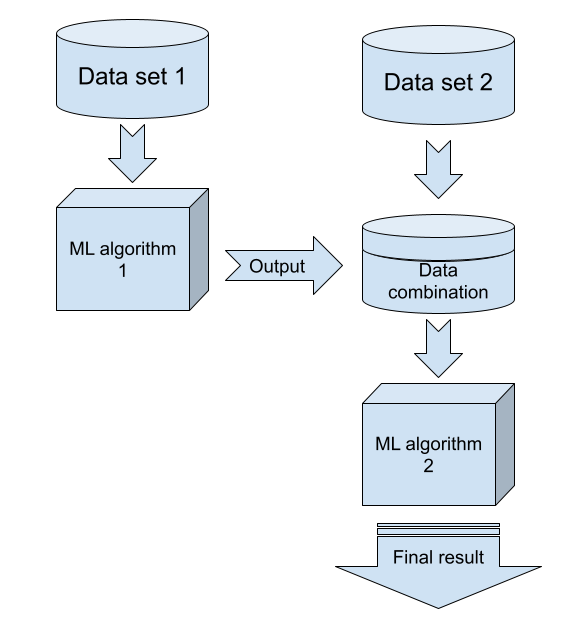
\includegraphics[width=0.5\textwidth,]{./appendices/hybrid-ml-model}
    \caption{Simplistic example of a hybrid machine learning model.
    The first algorithm learns from the initial data,
        and the results are used with a second data set to train another algorithm.
        \label{fig:hybrid-ml-model}}
\end{figure}

It is not feasible to use anomaly detection on its own to estimate ticket amounts
as plain sum of anomalies detected
is not correlating with tickets received.
Using pure statistical values of the log data
such as log rows per day
would possibly give some results with a single algorithm,
but only if the amount of log events correlates strongly with tickets received.
We can, however,
amplify our ticket estimating algorithm with anomaly feature values.
As we first count the anomaly numbers with the anomaly detection algorithm
and use the statistical features of the results in another algorithm,
like regression algorithm,
we get more relative information to use
when creating the final ticket number estimations.
This is explained in more detail
later in section~\ref{subsec:pipe-random-delay-and-timeframe-compression}.


%% ************************************************************************************************************


\subsection{HML phase 1: PCA-based anomaly detection algorithm}\label{subsec:pipe-pca-ada-input-output}


%% ............................................................................................................

\subsubsection*{PCA-ADA input feature formatting}
In Azure ML Studio, the only selectable module for
anomaly detection is the PCA-based anomaly detection
algorithm (PCA-ADA), which is explained in section~\ref{subsec:bg-pca-ada}.
However,
with textual input like logs
it can be used in at least two ways.

First,
input data can be fed to
the algorithm trainer as is,
letting the PCA-ADA component
do the work without further modifying the log rows.
This way,
the component tries to recognize the anomalies
based on all the information included in the row.
Practically this means,
that the component processes data in textual format
making each row in the input
a feature as a whole to consider.
As we discussed in the section~\ref{subsec:meth-data-anonymization},
unique values should be removed from the log rows
and the data should be somewhat clean.
PCA should be able to find similar values
and create anomaly score with purely textual features.
However,
it is probable that with a single word change on a message feature,
PCA defines two rows as completely different.

Second option is to convert the textual features into numerical features.
This can be done
either with the "Extract N-Gram Features from Text" component,
or the "Feature Hashing" component which uses n-gram feature extraction behind the scenes.
With n-gram feature extracting,
as explained in the section~\ref{subsec:bg-ngram-features-and-hashing},
each word or n-gram is converted to a number of said instance found on the row being processed,
and each row can be presented as a sequence of numbers
indicating the number of those features.

An N-gram feature can in addition have a weight
based on the frequency the n-grams appear
in the entire data.
Different weights usable in Azure ML component
are listed in table~\ref{tab:n-gram-weights}.
During this study,
only binary weight was used,
so it is possible that improved results could have been acquired with a different weight method.

\begin{table}[htb]
    \begin{tabularx}{\textwidth}{|L{0.25\textwidth}|X|}
        \hline
        \textbf{N-gram weight}  & \textbf{Explanation}       \\ \hline
        Binary Weight       & Assigns a binary presence value to the extracted n-grams. The value for each n-gram is 1 when it exists in the document, and 0 otherwise.     \\ \hline
        TF Weight           & Assigns a term frequency (TF) score to the extracted n-grams. The value for each n-gram is its occurrence frequency in the document.                \\ \hline
        IDF Weight          & Assigns an inverse document frequency (IDF) score to the extracted n-grams. The value for each n-gram is the log of corpus size divided by its occurrence frequency in the whole corpus. \verb-IDF = log of corpus_size / document_frequency-        \\ \hline
        TF-IDF Weight       & Assigns a term frequency/inverse document frequency (TF/IDF) score to the extracted n-grams. The value for each n-gram is its TF score multiplied by its IDF score.      \\ \hline
    \end{tabularx}
    \caption{Statistic metrics of the time frame compression that are considered possibly useful for ML algorithm.~\cite{azure2021ngramfeature}}
    \label{tab:n-gram-weights}
\end{table}

As stated,
a vast dictionary of n-grams demands resources from the ML computing instances
as every new n-gram in the dictionary adds another column to the training dataset.
To reduce the amount of memory needed,
the "Feature Hashing" component can be used.
By hashing the n-gram features,
the amount of resources needed by the pipeline
can be significantly reduced.
Feature hashing allows us to use the entire amount of data as an input
if feature hashing parameters are tuned enough.
However,
as discussed in the section~\ref{subsec:bg-ngram-features-and-hashing},
the greater the compression is,
the more information is lost
to reduce the need for resources.

Before the n-gram operations,
the textual data can be preformatted in Azure ML Studio
with \enquote{Preprocess text} -component.
This component includes several options to choose from
in order to clean text to more processable form.
Most useful options to select from are
\textit{stop word removal} (which removes uninformative words such as "the", "is" and "and"),
\textit{lemmatization} (which converts words to their canonical form,
for example "bigger mice eating" to "big mouse eat"),
\textit{detect sentence} (which inserts a sentence boundary symbol
to help algorithm text analysis),
\textit{text case normalization} (which normalizes all characters to lower case
to reduce the number of different words when first letter is capitalized),
and various \textit{character removals} (which range from number, special character, and duplicate character,
to url and email address removal possibilities).
Text preprocessing usually helps to reduce the number of features
when text is used in n-gram feature extraction and feature hashing.
Most of the options, however,
do not work well with other languages than English,
which might create issues with this study case
as logs contain a mixed amount of English and Finnish words.~\cite{azure2021preprocess}

In the end,
the need for memory proved problematic
and pure n-gram feature extracting forced us
to reduce the data size to only 2\%
in order to finish the algorithm training pipeline.
This amount was considered to be too low
for reliable algorithm training results.
Still,
all variations of input feature formatting were tested
to see how much possible shortcomings would affect the results.
More about the memory issue is discussed
in the section~\ref{subsec:res-memory-issues}.


%% ............................................................................................................


\subsubsection*{PCA output and anomaly probability}

The output values of the PCA-ADA component,
as explained in the section~\ref{subsec:bg-pca-ada},
are normalized so the values range between 0 and 1.
This anomaly probability value
is the main output of hybrid ML phase 1.
Based on our initial hypothesis,
that each anomalous event in the log
is linked to a real life support ticket received,
the bigger a single anomaly probability value is for a log row,
the more likely is that the row is related to a ticket inducing event.
Further processing steps of the output values
are discussed later in the section~\ref{subsec:pipe-random-delay-and-timeframe-compression}.

%% ************************************************************************************************************


\subsection{Unconventional training approach}\label{subsec:pipe-unconventional-training}

As stated in section~\ref{subsec:bg-machine-learning},
the approach we attempt in this study is,
if expression is allowed, unorthodox.
Typically,
the data points used in ML algorithm training and validating
should always be different.
Acting otherwise leads to algorithm processing with
same data it was trained with,
thus creating a situation
where algorithm already knows what to do with the current data point.
If the results were validated after this
the algorithm would get an unreliably good score
as it had the validation data already in the training phase.
This could be compared to
giving some right answers to students during a test
and scoring test results as if no help was given.
However,
due to the nature of the study problem and contents of the data,
it was decided to test whether bending this rule
would provide better results in algorithm training.

The large amount of data was enough
to cause issues with memory.
Although this problem was succesfully circumvented,
the hybrid approach and the time frame compression
(discussed later in section~\ref{subsec:pipe-random-delay-and-timeframe-compression})
resulted in a significant data loss in phase 2.
As a general rule of thumb in ML training,
only 20--30\% of the data is used to validate the algorithm.
With the hybrid ML approach,
the validation results in phase 1
are what actually form the data used in phase 2.
This data is further compressed to time frame groups
leading to only a few dozen data points in phase 2 ML training
compared to millions of rows in phase 1.

Because of the way the PCA-based anomaly detection algorithm works,
the over-lapping data points are not as big of an issue
as it would be with other types of algorithms
like regression algorithms.
This is why we could use part of the data
for training the anomaly detection algorithm as usual
and then use all the data available for validation
without overfitting the algorithm,
which happens when algorithm fits to the training data well,
but cannot generalize with new data~\cite{wang2016machine}.
Also, because the main forecasting functionality comes in the phase 2,
overfitting in phase 1 may not cause issues.

To verify if this unconventional training method gives good results without issues,
the trained algorithms were tested with new production data
that had zero overlapping data points with training and validation data.
This training method was also compared to a traditionally trained algorithm
to see the differences in results of both training styles.
This way we were able to compare different training approaches
to determine the best overall pipeline structure.

Kind of informal mention considering
the traditional training approach in our study case
is the data splitting of the log data for algorithm training.
Because of the hybrid model,
and the data consisting of log rows,
we cannot make a random split for the training and validation data
as is usually done.
Purely for training
the random splitting can be done,
but if data in phase 1 is split randomly for validation,
some anomalous rows could be skipped from a time frame
that would be crucial information for the estimations in phase 2.
This is why we must make sure the possible data splitting for validation data
is chronological in phase 1.


%% ************************************************************************************************************

\subsection{Input data random delay and time frame compression}\label{subsec:pipe-random-delay-and-timeframe-compression}

As mentioned previously in section~\ref{sec:introduction},
it takes time for a bank clerk to notice the error in the RPA process,
send a technical support ticket considering the issue,
and for the support team to redirect the request to the corresponding developer team.
As several steps of human interaction and workday schedules
are in between the event of logging and ticket receiving,
the random delay of such may span from hours to days.
Random delay in input data features
is not an unusual aspect in time-series forecasting.
Time-series in the context of ML
refers to data features that vary over time
and can be affected by past values.~\cite{palma2016time}
As an example,
an ML algorithm could try to predict future weather
based on measured temperature and air pressure.
Both these features change over time
and also affect their own future values.

This study, however,
is not about time-series
because the majority of the log rows
are not affected by previously logged events.
As random delay of such
does not seem to be trivial to take into account
with ML algorithms,
a simple method to solve this was used
where log rows were grouped by time stamp
into certain time frame groups.
We call this method \enquote{time frame compression method}.

Time frame compression means,
that in order to eliminate the effects of random delay
we compress some features into a certain time frame
at least as long as the longest estimated delay.
Simply put,
if we count possible anomalies during one hour of log,
we cannot compare this number to actual tickets received
at the same hour or the next.
What we can do,
with time frame compression,
is that we count some statistical values of anomaly estimates,
for example, the mean and median values of a week,
and then compare these numbers with the tickets received
during the same week.
Statistically important and thus compressible features of a time frame
were determined to be the log row count,
amount of unique job IDs, and anomaly probability metrics.

The amount of log rows describes
how many logged issues occured in a time frame.
Alone,
this feature may not give much insight
as the amount of logs is possibly not linearly comparable
to the amount of tickets received.
Combined to other statistical metrics
it may, however,
provide additional value for ticket forecasting.
Job ID is the identification information of a specific RPA automation execution run.
It means,
that the job ID is not unique for each log row,
but it binds together all the log entries on the same RPA automation execution.
By counting the amount of unique job IDs in a time frame
we can get insight about the amount of automation jobs executed during the time frame.
This metric is important with the total row count:
low number of unique jobs with high number of total rows
indicates that plenty of loggable events and possible errors happened during the time frame,
whereas high number of unique jobs combined to low number of rows
imply that not much happened (or perhaps executions were completely crashed).

By the original hypothesis,
anomalies in the logs are linked closely to the support tickets received.
The anomaly detection algorithm produces a probability value of
how strongly a row is considered to be an anomaly,
thus,
the mean and median values of the anomaly probabilities in a time frame
indicate how anomalous all the executions within a time frame have statistically been.
However,
when compressing the anomaly probability metrics in a time frame,
some information is bound to be lost.
The mean and median values do not provide information
about the anomaly probability value distribution.
There may be few very high values and a lot of low probabilities,
and it would lead to the same mean value
as if there were a lot of slightly higher probabilities and just few very low values.
By adding more statistical values
we can reduce the loss of information caused by time frame compression.
If the original hypothesis is correct,
the most relevant anomaly values are the highest anomaly probabilities.
Thus,
calculating higher quantiles and the amount of values exceeding them
should improve the estimation abilities of the algorithm.

\begin{table}[htb]
    \begin{tabularx}{\textwidth}{|L{0.4\textwidth}|X|}
        \hline
        \textbf{Statistic feature}  & \textbf{Explanation (in time frame)}       \\ \hline
        LogRowCount              & Number of rows/instances overall           \\ \hline
        UniqueJobIDs             & Amount of unique job IDs                   \\ \hline
        AnomalyProbabilityMean   & Mean value of anomaly probabilities        \\ \hline
        AnomalyProbabilityMedian & Median value of anomaly probabilities      \\ \hline
        AnomalyQuantile90        & 90-quantile value of anomaly probabilities \\ \hline
        AnomalyCountOverQ90 & Number of instances with anomaly probability over 90-quantile \\ \hline
    \end{tabularx}
    \caption{Statistic metrics of the time frame compression that are considered possibly useful for ML algorithm.}
    \label{tab:statistic-features}
\end{table}

In table~\ref{tab:statistic-features},
all the statistic metrics considered interesting and valuable
from time frame compression of the log rows
are listed with short explanation.
In the pipeline,
the statistical values are calculated
using the R-script executing component.
An example of such script executed by the "Execute R Script" component
is presented in appendix~\ref{sec:app-r-script}.


%% ************************************************************************************************************


\subsection{HML phase 2: Regression based estimating}\label{subsec:pipe-regression-estimating}

With the time frame compressed values
formed from the algorithm results in the phase 1,
we move on to the second phase in our HML pipeline
to estimate the ticket count.
Our second part of the data,
the technical ticket timestamps,
are compressed in same way as the result data in phase 1.
This time, however,
the timestamp data gets compressed
into a count of tickets received in the defined time frame.
Now we have a comparable feature
that is usable by regression algorithms.

Azure ML Studio has six regression algorithms usable.
One of them,
\textit{Fast Forest Quantile Regression},
is used to explain the distribution of value being predicted.\cite{azure2021fastforestquantile}
In our case, however,
this is does not provide any use for us
as we are predicting the ticket count per time frame.
The distribution of tickets on each time frame is irrelevant.

The remaining five algorithms are presented below:
\begin{enumerate}
    \item Linear regression~\cite{azure2021linear}
    \item Boosted decision tree regression~\cite{azure2022boosteddecisiontree}
    \item Decision forest regression~\cite{azure2021decisionforest}
    \item Neural network regression~\cite{azure2021neuralnetwork}
    \item Poisson regression~\cite{azure2021poisson}
\end{enumerate}

Linear regression is the simplest one,
and even though it can be easily explained with the least square principle
explained in the section~\ref{subsec:bg-regression-ml},
linear regression component is capable of more advanced methods,
such as gradient descent.
Poisson regression works only for Poisson distributed data.
As the distribution of the anomalies or ticket inducing log events is not certain,
we cannot rule this method out before seeing the results.

Other components with a \textit{tree} or \textit{forest} in their name
are based on the same algorithm model called \textit{decision trees}.
Decision trees are models
which run a series of simple tests
for all data points in each branching node.
The data is moved on like water along the tree from trunk to branches
until it reaches the leaf node which marks the decision-making point.
When multiple trees are placed in serial,
the decision tree becomes a forest.~\cite{azure2021decisionforest}

When decision searching tree branches do not trickle from few to many
but the flow can contract and widen again,
or multiple nodes can reach same child nodes,
the model becomes a neural network.

All of these regression algorithm models
were tested and their results validated with new data
in order to find the one with the most promising results.


%% ************************************************************************************************************


\subsection{Pipeline branching}\label{subsec:pipe-branching}

In order to find the best possible combination of components,
all different combinations must be compared.
As the pipeline is structured in a tree-like flow,
each node which includes more than one possible choices
diverges the pipeline into branches.
Several diverging points have been mentioned before in this study,
and in this section we join the information together.

First,
the error message used to calculate the anomaly probability of a log row
had two options.
We could either use simple \textit{message},
or more verbose \textit{rawmessage}.
This textual data could be fed to the ADA-component in several forms.
Most straightforward way was using textual data without any preformatting or modification.
Text could also be run through \enquote{Preprocess text} -component.
N-gram features could have been extracted from the original or preprocessed text
and these features could have been used instead.
Instead of n-gram features,
textual data could be converted to numeric
also with \enquote{Feature Hashing} -component.
After getting the ADA-component results,
the anomaly probabilities were compressed with R-code or SQL.\@
This concludes the phase 1.

In the next phase,
branching of the pipeline was due to
comparing results without the anomaly probability values calculated in phase 1,
and then utilizing different regression algorithms in phase 2.
In practice this means
that in order to validate the results against our initial hypothesis,
we used pure statistical log data,
such as row count and unique job ID count
without anomaly probabilities,
to determine whether anomaly metrics provided any insight regarding the ticket data.
When using n-gram features or hashed features,
these additional column features were also included for this comparison
as forming them does not depend on the anomaly properties of the log instance.

Each branching step, or layer,
multiplies the amount of comparable values used in final comparison
that would determine the best possible pipeline combination.
These layers are simplified in the table~\ref{tab:ml-pipeline-branching}.

\begin{table}[htb]
    \centering
    \begin{tabularx}{\textwidth}{|L{0.3\textwidth}|L{0.45\textwidth}|X|}
        \hline
        \textbf{Branching node}           &
        \textbf{Options}                 &
        \textbf{Divergent count} \\ \hline
        Input text column                  & \begin{tabular}[c]{@{}l@{}}message \\ rawmessage\end{tabular}                 & 2                        \\ \hline
        Text preprocess                    & \begin{tabular}[c]{@{}l@{}}Yes\\ No\end{tabular}                              & 2                        \\ \hline
        Numeric conversion                 & \begin{tabular}[c]{@{}l@{}}No\\ N-gram Feature\\ Feature Hashing\end{tabular} & 3                        \\ \hline
        ADA training                       & \begin{tabular}[c]{@{}l@{}}Unconventional \\ Proper\end{tabular}              & 2                        \\ \hline
        Validation without anomaly metrics & \begin{tabular}[c]{@{}l@{}}Yes\\ No\end{tabular}                           & 2                        \\ \hline
        Regression algorithms &
        \begin{tabular}[c]{@{}l@{}}
            Linear regression\\
            Boosted decision tree regression \\
            Decision forest regression \\
            Neural Network Regression \\
            Poisson regression \\
            \end{tabular}
        &   5 \\ \hline
    \end{tabularx}
    \caption{Pipeline divergent layers}
    \label{tab:ml-pipeline-branching}
\end{table}

The divergent count implies the number of branches
diverging from the previous component.
The total count of branch ends, or leaves,
would then be the multiplication of all divergent counts,
totaling to 240 comparable pipeline combinations.
Moreover,
n-gram feature extraction and feature hashing
have several tunable parameters
that strongly influence the end results of the algorithm training.
To reduce this amount when considering the best possible pipeline,
we simplified this by narrowing down the options
based on initial test run results of some of the divergent options.

For example,
n-gram feature component suffered greatly from the memory problem
(which we discuss more in section~\ref{subsec:res-memory-issues}),
and the data amount that the \textit{Extract N-Gram Features from Text} -component was able to handle
comprised of only 2\% of the original data.
This was deemed as too small amount for training an ML algorithm
as it would be extremely likely with 98\% of the data skipped
that also possible rows relevant to the ticket anomalies
would get trimmed out too.

The flowchart of pipeline with branching options visualized
is illustrated in figure~\ref{fig:pipeline-flowchart}.
The final pipeline structure used for result acquiring
can be seen in the appendix~\ref{sec:app-final-pipeline-structure}.
\begin{figure}[htb]
    \centering
    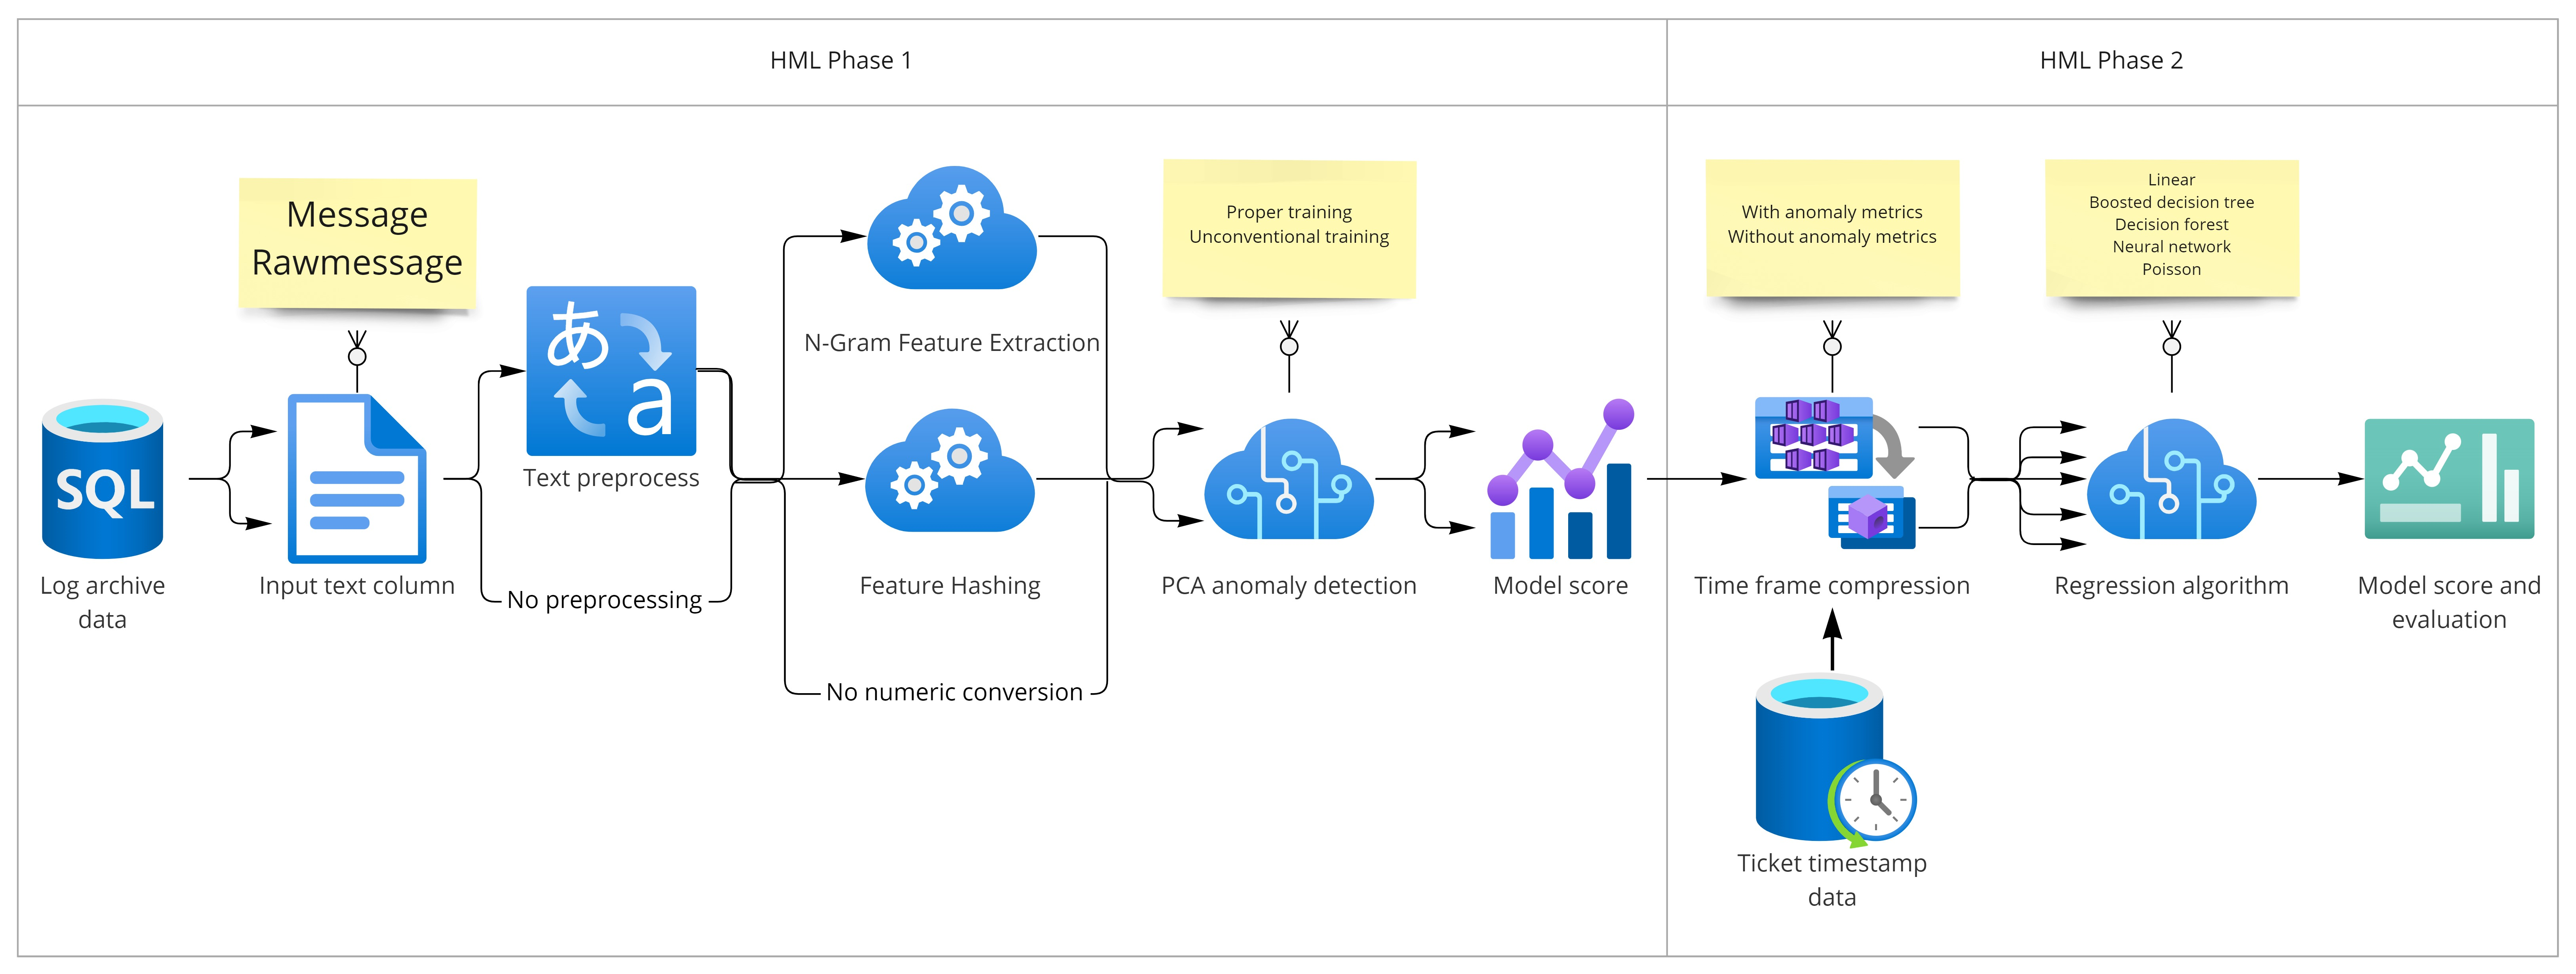
\includegraphics[width=\textwidth]{./appendices/pipeline-flowchart.jpg}
    \caption{Pipeline flowchart with branching steps illustrated.
    HML phase boundaries are made visible for clarity.
    \label{fig:pipeline-flowchart}}
\end{figure}


%% ************************************************************************************************************


\subsection{Comparable metrics}\label{subsec:pipe-comparable-metrics}

In previous sections we have discussed of different approaches that could be used
to get the best results from the ML training.
In order to find the best possible combination of components,
we must compare different results,
and for this we need comparable metrics.
After training,
Azure regression algorithms are scored with a validation data.
The final output from this is a numeric \textit{Scored Labels} feature.
In our study case,
this value is what algorithm estimates the ticket count on the time frame to be.
Next,
the \textit{Evaluate Model} component calculates a few evaluation metrics
to be used for result comparison.
These metrics for regression algorithm are listed
in table~\ref{tab:comparable-metrics}.

\setlength{\tabcolsep}{5pt}
\begin{table}[htb]
    \begin{tabularx}{\textwidth}{|L{0.35\textwidth}|X|}
        \hline
        \textbf{Name of the metric}             & \textbf{Explanation}  \\ \hline
        Mean Absolute Error (MAE)               & Measures how close the predictions are to the actual outcomes;
            thus, a lower score is better. \\ \hline
        Root Mean Squared Error (RMSE)          & Creates a single value that summarizes the error in the model.
            By squaring the difference, the metric disregards the difference between over-prediction and under-prediction. \\ \hline
        Relative Squared Error (RSE)            & Normalizes the total squared error of the predicted values
            by dividing by the total squared error of the actual values. \\ \hline
        Relative Absolute Error (RAE)           & The relative absolute difference between expected and actual values;
            relative because the mean difference is divided by the arithmetic mean. \\ \hline
        Coefficient of Determination (CoD)      & Often referred to as $R^{2}$,
            represents the predictive power of the model as a value between 0 and 1.
            Zero means the model is random (explains nothing);
            1 means there is a perfect fit.
            However, caution should be used in interpreting $R^{2}$ values,
            as low values can be entirely normal and high values can be suspect. \\ \hline
    \end{tabularx}
    \caption{Comparable metrics provided by \textit{Evaluate Model} component for regression algorithm.\cite{azure2021evaluate}}
    \label{tab:comparable-metrics}
\end{table}

Our goal is to find a connection
between the log anomalies and the ticket timestamps.
Our initial hypothesis suggested
that the most anomalous events in the logs
would be more related to the ticket events than other rows.
Thus,
by comparing the algorithm evaluation metrics
to the metrics produced by the neighboring pipeline branch
where anomaly probabilities has been removed,
we should find the best algorithm where evaluation values
are significantly better than the same algorithm without those anomaly values.
This would prove,
that the anomaly probability values improve the algorithm estimations
indicating that the hybrid algorithm combination has indeed found the connection
between anomalies and ticket timestamps.
This will also be our logical basis when selecting certain algorithms for further tests.




\clearpage